\documentclass[letterpaper]{article}
\usepackage[utf8]{inputenc}
\usepackage[T1]{fontenc}
\usepackage{lmodern}
\usepackage{enumerate}
\usepackage{xcolor}
\usepackage{graphicx}
\usepackage{multicol}
\usepackage{amsmath}
\usepackage{tabularx}
\usepackage{multirow}
\usepackage[spanish,es-nodecimaldot, es-tabla]{babel}
\usepackage{wrapfig}
\usepackage[rightcaption]{sidecap}
\graphicspath{ {./} }
\usepackage{amssymb}
\usepackage{setspace}
\usepackage{fancyhdr}
\usepackage[left=2.5 cm,right=2.5 cm, top=2.5 cm, bottom=2.5 cm]{geometry}
\usepackage{float}
\usepackage{afterpage}
\usepackage{tikz}
\usetikzlibrary{arrows.meta, decorations.pathreplacing}

% Configuración de encabezado y pie de página
\pagestyle{fancy}
\fancyhf{} % Limpia encabezado y pie
\fancyhead[R]{\small Estudiante de posgrado, Centro de Investigaciones en Óptica \\ Metrología Óptica}
\fancyfoot[C]{\thepage} % Número de página centrado
\renewcommand{\headrulewidth}{0pt} % Quita la línea bajo el encabezado
\renewcommand{\footrulewidth}{0pt} % Quita línea sobre pie de página

\begin{document}
	
	\begin{center}
		\Large \textbf{PERFILOMETRÍA DE PROYECCIÓN DE FRANJAS (FPP)}
	\end{center}
	
	\begin{center}
		Jonathan Francisco Rojas Martínez\\
		jonathan.frm@cio.mx\\
		09/07/2026\\
		Centro de Investigaciones en Óptica\\
		Loma del Bosque 115, Lomas del Campestre, León, Gto, C.P. 37150
	\end{center}
	
	\begin{center}
		{\Large \textbf{Resumen}}
	\end{center}
	
	\noindent
	En este trabajo se aplicó la técnica de Perfilometría de Proyección de Franjas (FPP) basada en el principio de triangulación óptica para la reconstrucción tridimensional de campo completo de una superficie. Mediante un proyector digital se iluminó el objeto con patrones de franjas sinusoidales y se adquirieron las imágenes deformadas con una cámara CCD. La topografía se extrajo utilizando un algoritmo de corrimiento de fase (\textit{Phase Shifting}) de 4 pasos, calculando la fase envuelta mediante la función arcotangente, seguido de un desenvolvimiento de fase (\textit{Phase Unwrapping}) para remover discontinuidades espaciales. Los resultados demostraron la viabilidad computacional y precisión de esta técnica no invasiva.
	
	\begin{multicols}{2}
		
		\section*{Introducción}
		
		El uso de la luz estructurada en la medición tridimensional de superficies se ha convertido en una herramienta indispensable en metrología óptica. Consiste en la proyección de patrones geométricos conocidos, como franjas sinusoidales, sobre una escena. El análisis de la distorsión que sufren estos patrones al incidir sobre el objeto permite recuperar su geometría tridimensional de manera no invasiva.
		
		Dentro de estas técnicas destaca la Perfilometría de Proyección de Franjas (FPP). Esta técnica permite calcular la altura $h(x,y)$ a partir de la fase óptica extraída de los patrones de intensidad registrados por una cámara ubicada a un ángulo $\alpha$ respecto al proyector. Para ello, se suele utilizar el método de corrimiento de fase (\textit{Phase Shifting}), proyectando varios patrones desfasados entre sí, lo que facilita aislar el término de fase mediante operaciones algebraicas, minimizando el impacto de la iluminación de fondo y las variaciones de reflectividad.
		
		\section*{Objetivos}
		
		\begin{itemize}
			\item Reconstruir la topografía 3D de un objeto de prueba mediante proyección digital de franjas.
			\item Implementar computacionalmente el algoritmo de corrimiento de fase de 4 pasos para la obtención de la fase envuelta.
			\item Comprender y aplicar el desenvolvimiento de fase para extraer el mapa continuo de altura.
		\end{itemize}
		
		\section*{Material y equipo}
		
		\begin{enumerate}
			\item Proyector digital LCD.
			\item Cámara CCD.
			\item PC con software de toma de imagenes y para procesamiento de estas.
			\item Objeto de prueba esférica.
			\item Monturas y bases mecánicas.
		\end{enumerate}
		
		\section*{Procedimiento}
		
		\begin{enumerate}[i)]
			\item Configurar la geometría del sistema: calibrar la distancia base $L$ y el ángulo $\alpha$ entre la cámara y el proyector.
			\item Generar computacionalmente 4 patrones de franjas sinusoidales con desfasajes de $\pi/2$ ($0, \pi/2, \pi, 3\pi/2$).
			\item Proyectar secuencialmente los patrones sobre el objeto de prueba y registrar las imágenes $I_1, I_2, I_3, I_4$.
			\item Utilizar un script en Python para procesar las imágenes, calculando la fase envuelta con la función matricial \texttt{np.arctan2(I4 - I2, I1 - I3)}.
			\item Aplicar un algoritmo de desenvolvimiento de fase para convertir la fase discontinua en una fase continua $\Phi(x,y)$.
			\item Calcular el desplazamiento lateral $u(x)$ y convertirlo en altura topográfica $z = h(x,y)$ aplicando las ecuaciones de triangulación óptica.
		\end{enumerate}
		
		\section*{Resultados y Análisis}
		
		El procesamiento computacional de los patrones de franjas adquiridos arrojó resultados consistentes con el modelo matemático de triangulación óptica. A continuación, se detalla el análisis de cada etapa del procesamiento:
		
		\begin{itemize}
			\item \textbf{Fase Envuelta:} El cálculo algebraico del algoritmo de corrimiento de fase de 4 pasos permitió extraer el argumento trigonométrico de la deformación. Como se observa en los resultados, la superficie del objeto presenta un patrón de fase definido; sin embargo, las regiones del fondo carentes de franjas estructuradas exhiben un severo ruido aleatorio (ruido de fase) debido a la nula modulación de la luz.
			
			\item \textbf{Máscara de Modulación:} Para evitar la propagación de errores durante el desenvolvimiento, se calculó una máscara booleana evaluando el contraste local de las franjas (umbralizado al 15\% del valor máximo). Esta máscara segmentó de manera robusta la región de interés (fondo válido y objeto). Físicamente, el algoritmo detectó y excluyó una pequeña zona en forma de media luna en el flanco izquierdo del objeto; esta exclusión es correcta y responde a una baja modulación local causada por la sombra (oclusión) de la proyección geométrica.
			
			\item \textbf{Fase Desenvuelta (Relieve 2D):} Al aplicar el algoritmo de \textit{unwrapping} exclusivamente sobre los píxeles validados por la máscara, se logró remover con éxito las discontinuidades de $2\pi$ radianes. El resultado es un mapa de gradiente continuo libre de artefactos de ruido, el cual es directamente proporcional a la topografía del objeto.
			
			\item \textbf{Topografía 3D (Escala Real):} Utilizando los parámetros de calibración del arreglo experimental (base $L = 171.0\text{ mm}$, distancia $LC = 670.0\text{ mm}$, y un periodo $p = 27.0\text{ mm}$), la fase continua fue mapeada a coordenadas métricas. El análisis espacial demuestra que el plano de referencia se mantiene constante alrededor de los $0\text{ mm}$ de elevación. Por su parte, la superficie de prueba exhibe una deformación máxima de aproximadamente $-55\text{ mm}$. La representación cóncava (valores negativos en el eje $Z$) es un resultado directo de la geometría de captura y refleja el signo del vector de desplazamiento lateral de las franjas proyectadas.
		\end{itemize}
		

		
		
		\section*{Cuestionario}
		\begin{enumerate}
			\item \textbf{A parte de FPP, mencione y describa brevemente otras técnicas de obtención de la forma.}\\
			Otras técnicas incluyen el Moiré de Sombras, donde se interpone una rejilla física cerca del objeto para generar patrones de interferencia de baja frecuencia; la visión estéreo binocular pasiva, que utiliza correspondencia geométrica entre dos cámaras simulando la visión humana; y los métodos de Tiempo de Vuelo (ToF) que miden el tiempo de retorno de un pulso de luz.
			
			\item \textbf{¿A qué se refiere cuando se habla de obtener la fase de un objeto deformado por franjas?}\\
			Se refiere a aislar el argumento trigonométrico (la fase óptica $\phi$) del patrón de intensidad capturado. Como la altura topográfica $h(x,y)$ induce un desplazamiento lateral $u(x)$ en las franjas proyectadas, este desplazamiento queda codificado directamente dentro de dicha fase para su posterior extracción espacial.
			
			\item \textbf{Desarrolle el método que usó para obtener la fase del objeto a partir de patrones.}\\
			Se implementó el algoritmo de corrimiento de fase (\textit{Phase Shifting}) de 4 pasos adquiriendo patrones desfasados en $\pi/2$. Las variaciones de reflectividad y luz de fondo se cancelan tomando las diferencias matemáticas $(I_4 - I_2)$ y $(I_1 - I_3)$. Computacionalmente, la fase envuelta se calcula en el rango $[-\pi, \pi)$ utilizando la función \texttt{arctan2((I4-I2), (I1-I3))}.
			
			\item \textbf{¿Qué consideraciones principales (como el efecto Gamma) se deben tener en el uso de luz estructurada?}\\
			Uno de los desafíos principales es el Efecto Gamma introducido por el proyector comercial, el cual incorpora una respuesta de intensidad no lineal que deforma el perfil senoidal puro agregando armónicos perjudiciales. Se debe corregir mediante software (LUT) o desenfocando ligeramente la lente del proyector. Además, es indispensable realizar una rigurosa calibración extrínseca/intrínseca (cámara-proyector) y considerar que los objetos muy especulares (brillosos) tienden a saturar la CCD.
		\end{enumerate}
		
		\section*{Conclusiones}
		La implementación del algoritmo de corrimiento de fase (Phase Shifting) de 4 pasos permitió recuperar exitosamente la topografía del objeto de prueba. Se comprobó que el cálculo de la fase envuelta es altamente susceptible al ruido óptico y de fondo; sin embargo, el uso de una máscara de modulación dinámica basada en el contraste de las franjas mitigó este problema. Como se observa en los resultados bidimensionales, el umbral logró discriminar efectivamente las áreas sin patrón estructurado. Asimismo, la máscara detectó una zona de baja modulación geométrica sobre la superficie del objeto (visible como un corte en forma de media luna), fenómeno que es físicamente atribuible a la sombra proyectada por la oclusión geométrica o a la saturación por reflexión especular.
		
		Al evaluar la reconstrucción métrica tridimensional, el mapeo de la fase desenvuelta a coordenadas físicas en milímetros demostró la viabilidad cuantitativa de la técnica de triangulación óptica para metrología de campo completo. El plano de referencia se mantuvo analíticamente estable alrededor de los $0\text{ mm}$, mientras que la superficie del objeto registró un desnivel máximo aproximado de $55\text{ mm}$. 
		
		Un hallazgo analítico a destacar en la representación 3D es la concavidad del objeto, graficado en el eje $Z$ negativo. Asumiendo que el objeto físico evaluado presentaba una geometría convexa, esta inversión topográfica evidencia empíricamente la convención de signos trigonométrica del sistema; el desplazamiento de fase lateral $u(x)$ resulta positivo o negativo dependiendo estrictamente de si la cámara se encuentra posicionada a la derecha o a la izquierda del eje óptico del proyector. En conclusión, el desarrollo y ajuste de estas rutinas computacionales en Python resultan indispensables para garantizar la fidelidad geométrica absoluta en el campo de la metrología óptica moderna.
		
		\section*{Bibliografía}
		\begin{enumerate}
			\item Documento de Apoyo: \textit{Técnicas de luz estructuradas}. Apuntes de Estudio CIO.
			\item Zhang, S. (2010). \textit{Recent progresses on real-time 3D shape measurement using digital fringe projection techniques}. Optics and Lasers in Engineering.
			\item Gorthi, S. S., \& Rastogi, P. (2010). \textit{Fringe projection techniques: Whither we are?}. Optics and Lasers in Engineering.
		\end{enumerate}
		
	\end{multicols}
	
	
	
	\begin{figure}[H]
		\centering
		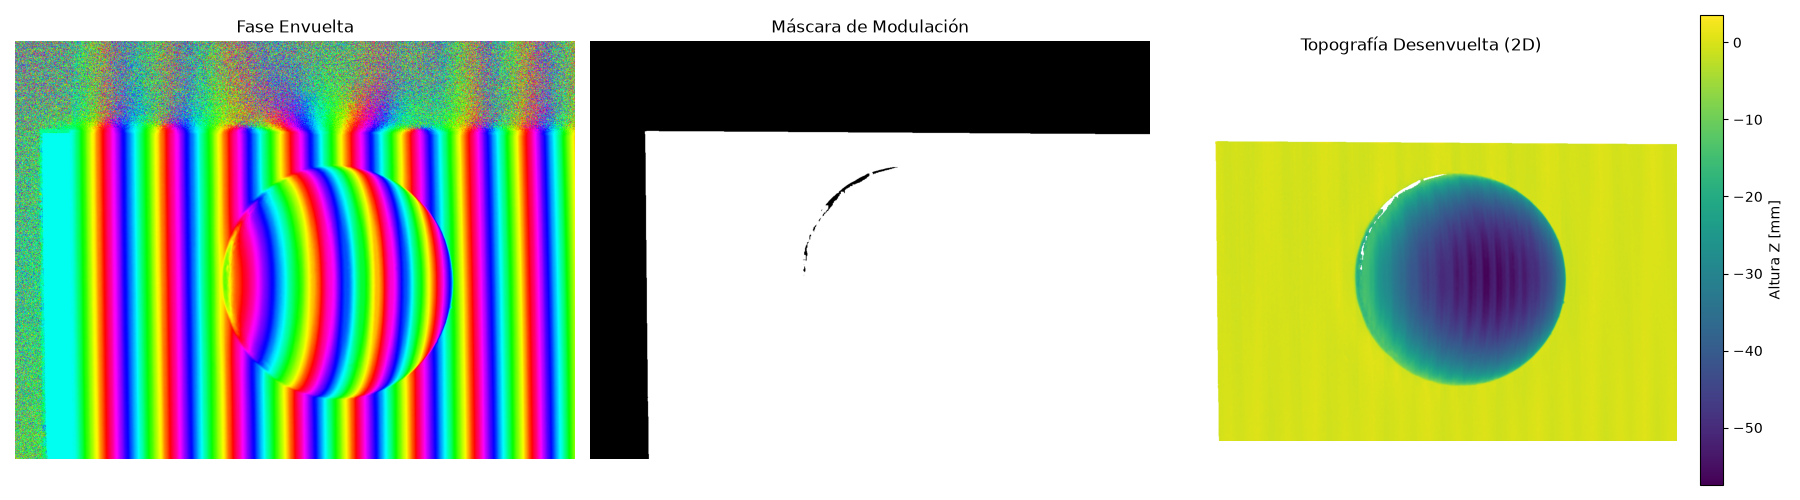
\includegraphics[width=\linewidth]{Analisis_antes_de_reconstruccion.png}
		\caption{Patrón de franjas sinusoidal deformado por el relieve tridimensional del objeto analizado y su fase envuelta.}
		\label{fig:franjas}
	\end{figure}
	
	\begin{figure}[H]
		\centering
		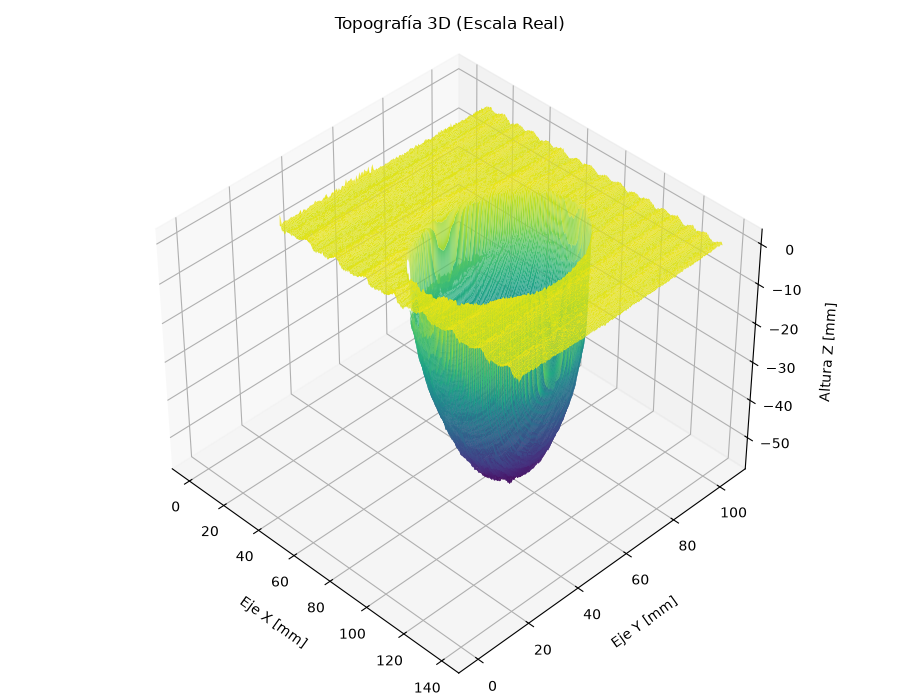
\includegraphics[width=\linewidth]{3D.png}
		\caption{Reconstrucción 3D del objeto visto mediante FPP.}
		\label{fig:fases}
	\end{figure}
	
\end{document}